% \section{Print Composer}\label{label_printcomposer}
\section{Composeur de carte}\label{label_printcomposer}

% when the revision of a section has been finalized, 
% comment out the following line:
% \updatedisclaimer

% The print composer provides growing layout and printing capabilities. It
% allows you to add elements such as the QGIS map canvas, legend, scalebar,
% images, and text labels. You can size, group and position each element and
% adjust the properties to create your layout. The result can be printed (also
% to Postscript and PDF), exported to image formats or to SVG.\footnote{Export
% to SVG supported, but it is not working properly with some recent QT4
% versions. You should try and check individual on your system} See a list of
% tools in table~\ref{tab:printcomposer_tools}:
Le composeur de carte fournit des fonctionnalités croissantes de mise en page et
d'impression. Il vous permet d'ajouter des éléments tels qu'un cadre de carte
QGIS, une légende, une échelle graphique, des images et des étiquettes. Vous
pouvez modifier la taille, grouper et positionner chaque élément et ajuster
leurs propriétés pour créer votre mise en page. Le résultat peut être imprimé
(ainsi qu'imprimé en Postscript et PDF), exporter dans un format d'image ou en
SVG.\footnote{L'export en SVG est géré, mais il ne fonctionne pas proprement
avec des versions récentes de QT4. Vous devez essayer et vérifier
indivuellement sur votre système] Voyez une liste d'outils dans le
tableau~\ref{tab:printcomposer_tools} :

% \begin{table}[h]\index{Print composer!tools}
\begin{table}[h]\index{Composeur de carte!outils}
\centering
% \caption{Print Composer Tools}\label{tab:printcomposer_tools}\medskip
\caption{Outils du Composeur de carte}\label{tab:printcomposer_tools}\medskip
 \begin{tabular}{|l|p{6.9cm}|l|p{6.9cm}|}
%  \hline \textbf{Icon} & \textbf{Purpose} & \textbf{Icon} &
%  \textbf{Purpose} \\
 \hline \textbf{Icône} & \textbf{Objectif} & \textbf{Icône} &
 \textbf{Objectif} \\
 
%  \hline 
\includegraphics[width=0.7cm]{mActionExportMapServer} & Export to an
% image format & 
\hline 
\includegraphics[width=0.7cm]{mActionExportMapServer}  & Exporter dans un
format d'image & 
%  
\includegraphics[width=0.7cm]{mActionSaveAsSVG} & Export print composition 
%  to SVG \\
 
\includegraphics[width=0.7cm]{mActionSaveAsSVG} & Exporter la composition en 
SVG \\
%  \hline 
\includegraphics[width=0.7cm]{mActionFilePrint} & Print or  export as
% PDF or Postscript &
 \hline 
\includegraphics[width=0.7cm]{mActionFilePrint} & Imprimer pu exporte
r comme PDF ou Postscript &
%  
\includegraphics[width=0.7cm]{mActionZoomFullExtent} & Zoom to  full extend
% \\

\includegraphics[width=0.7cm]{mActionZoomFullExtent} & Zoom à l'étendue
maximale\\
%  \hline 
\includegraphics[width=0.7cm]{mActionZoomIn} & Zoom in & 
%  
\includegraphics[width=0.7cm]{mActionZoomOut} & Zoom out \\
\hline 
\includegraphics[width=0.7cm]{mActionZoomIn} & Zoom in &
 
\includegraphics[width=0.7cm]{mActionZoomOut} & Zoom out \\
%  \hline 
\includegraphics[width=0.7cm]{mActionDraw} & Refresh view &
%  
\includegraphics[width=0.7cm]{mActionAddRasterLayer} & Add new map from QGIS
% map canvas \\
 \hline 
\includegraphics[width=0.7cm]{mActionDraw} & Rafraichie la vue &
 
\includegraphics[width=0.7cm]{mActionAddRasterLayer} & Ajouter une nouvelle 
carte à partir du cadre de carte de QGIS \\
%  \hline 
\includegraphics[width=0.7cm]{mActionSaveMapAsImage} & Add Image to 
%  print composition &
 \hline 
\includegraphics[width=0.7cm]{mActionSaveMapAsImage} & Ajouter une image
au composeur de carte &
%  
\includegraphics[width=0.7cm]{mActionLabel} & Add label to print composition
% \\

\includegraphics[width=0.7cm]{mActionLabel} & Ajoute des étiquettes à la
composition de carte \\
%  \hline 
\includegraphics[width=0.7cm]{mActionAddLegend} & Add new legend to 
%  print composition & 
\hline 
\includegraphics[width=0.7cm]{mActionAddLegend} & Ajoute une nouvelle 
légende à la composition de carte &
%  
\includegraphics[width=0.7cm]{mActionScaleBar} & Add new scalebar to print
%  composition\\
 
\includegraphics[width=0.7cm]{mActionScaleBar} & Ajoute une barre
d'échelle graphique à la composition de carte\\
%  \hline 
\includegraphics[width=0.7cm]{mActionSelectPan} & Select/Move item in 
%  print composition &
\hline 
\includegraphics[width=0.7cm]{mActionSelectPan} & Sélectionne/déplace les
objets dans la composition de carte &
%  
\includegraphics[width=0.7cm]{mActionMoveItemContent} & Move content within
%  an item \\

\includegraphics[width=0.7cm]{mActionMoveItemContent} & Déplace le contenu dans
un objet \\
%  \hline 
\includegraphics[width=0.7cm]{mActionGroupItems} & Group items of 
%  print composition & 
 \hline 
\includegraphics[width=0.7cm]{mActionGroupItems} & Groupe les objets de
la composition de carte & 
%  
\includegraphics[width=0.7cm]{mActionUngroupItems} & Ungroup items of print 
%  composition \\
 
\includegraphics[width=0.7cm]{mActionUngroupItems} & Désolidaise les objets de
la composition de carte \\
%  \hline 
\includegraphics[width=0.7cm]{mActionRaiseItems} & Raise selected
%  items in print composition &
 \hline 
\includegraphics[width=0.7cm]{mActionRaiseItems} & Passe les objets par
dessus dans la composition de carte &
%  
\includegraphics[width=0.7cm]{mActionLowerItems} & Lower selected items 
%  in print composition \\

\includegraphics[width=0.7cm]{mActionLowerItems} & Passe les objets par dessous
dans la composition de carte \\
%  \hline 
\includegraphics[width=0.7cm]{mActionMoveItemsToTop} & Move selected
%  items to top & 
 \hline 
\includegraphics[width=0.7cm]{mActionMoveItemsToTop} & Déplace les
objets sélectionnés tout en haut & 
%  
\includegraphics[width=0.7cm]{mActionMoveItemsToBottom} & Move selected
%  items to bottom \\
 
\includegraphics[width=0.7cm]{mActionMoveItemsToBottom} & Déplace les
objets sélectionnés tout en bas \\
\hline
\end{tabular}
\end{table}

% To access the print composer, click on the
% \toolbtntwo{mActionFilePrint}{Print} button in the toolbar or choose
% \mainmenuopt{File} > \dropmenuopttwo{mActionFilePrint}{Print Composer}.
Pour accéder au composeur de carte, cliquez sur le bouton
\toolbtntwo{mActionFilePrint}{Imprimer} dans la barre d'outils ou choisissez
\mainmenuopt{Fichier} > \dropmenuopttwo{mActionFilePrint}{Composeur de carte}.

% \subsection{Using Print Composer}\label{label_useprintcomposer} 
\subsection{Utiliser le Composeur d'Impression}\label{label_useprintcomposer} 


% Before you start to work with the print composer, you need to load some 
% raster and vector layers in the QGIS map canvas and adapt their properties 
% to suite your own convinience. After everything is rendered and symbolized to 
% your liking you click the \toolbtntwo{mActionFilePrint}{Print Composer} icon.
Avant de démarrer à travailler avec le composeur de carte, vous devez charger
certaines couches raster et vecteurs dans la fenêtre de carte de QGIS et 
adapter leurs propriétés pour qu'elles vous conviennent. Après que tout soit
rendu et symbolisé comme vous le souhaitez, cliquez sur l'icône 
\toolbtntwo{mActionFilePrint}{Composeur de carte}.

\begin{figure}[ht]
   \begin{center}
%    \caption{Print Composer\nixcaption}
    \caption{Composeur de carte\nixcaption}
\label{fig:print_composer_blank}\smallskip
   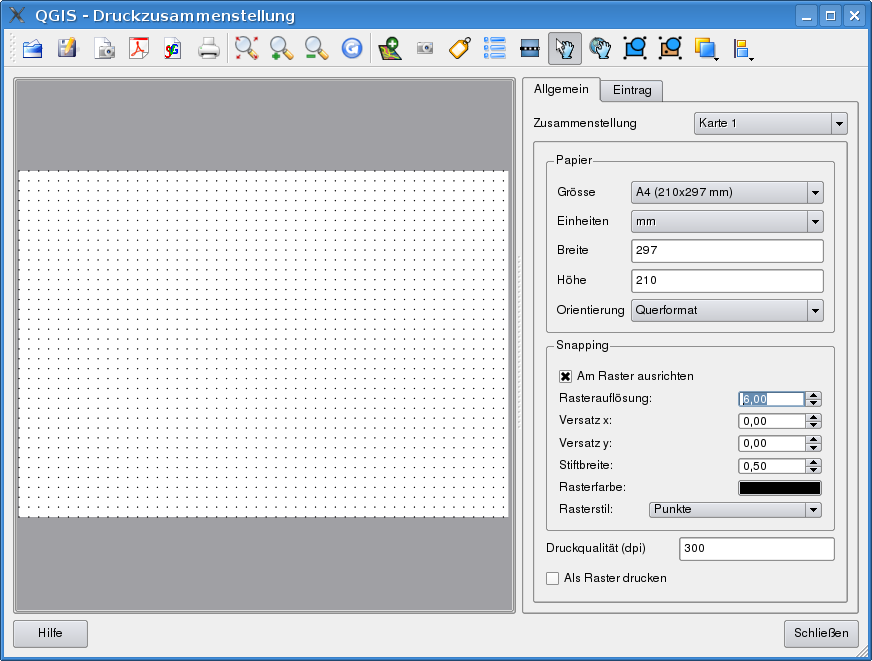
\includegraphics[clip=true, width=\textwidth]{print_composer_blank}
\end{center}
\end{figure}

% Opening the print composer provides you with a blank canvas to which you can 
% add the current QGIS map canvas, legend, scalebar, images and text. Figure
% \ref{fig:print_composer_blank} shows the initial view of the print composer 
% before any elements are added. The print composer provides two tabs:
Ouvrir le composeur de carte vous affiche un cadre vide auquel vous pouvez
ajouter un cadre de la carte actuelle de QGIS, une légende, une échelle
graphique, des images et du texte. La figure \ref{fig:print_composer_blank}
montre la vue initiale du composeur de carte avant qu'un élément ne soit
ajouté. Le composeur de carte affiche deux onglets :

\begin{itemize}
% \item The \tab{General} tab allows you to set paper size, orientation, and
% the print quality for the output file in dpi.
\item l'onglet \tab{Général} vous permet de définir la taille du papier,
l'orientation et la qualité d'impression pour le fichier de sortie, en dpi.
% \item The \tab{Item} tab displays the properties for the selected map
% element. Click the \toolbtntwo{mActionSelectPan}{Select/Move item} 
% icon to select an element (e.g. legend, scalebar or label) on the canvas. 
% Then click the Item tab and customize the settings for the selected element.
\item L'onglet \tab{Item} affiche les propriétés pour l'élément de la carte
sélectionnée. Cliquez sur l'icône
\toolbtntwo{mActionSelectPan}{Sélectionner/Déplacer l'objet}  pour sélectionner
un élément (par exemple l'échelle graphique ou une étiquette) dans le cadre.
Puis cliquez sur l'onglet Item et personnalisez les paramètres pour l'élément
sélectionné.
\end{itemize}

% You can add multiple elements to the composer. It is also possible to have 
% more than one map view or legend or scalebar in the print composer canvas. 
% Each element has its own properties and in the case of the map, its own 
% extent.
Vous pouvez ajouter de multiples éléments au composeur. Il est également
possible d'avoir plus d'une vue de carte, légende ou échelle graphique dans le
cadre du composeur de carte. Chaque élément possède ses propres propriétés et
dans le cas de la carte, sa propre étendue.

% \subsubsection{Adding a current QGIS map canvas to the Print Composer}
\subsubsection{Ajouter une carte en cours dans QGIS au Composeur d'Impression}

% To add the QGIS map canvas, click on the
% \toolbtntwo{mActionAddRasterLayer}{Add new map from QGIS map canvas} button in
% the print composer toolbar and drag a rectangle on the composer canvas with
% the left mouse button to add the map. You will see an empty box with a
% \textit{"Map will be printed here"} message. To display the current map,
% choose \selectstring{Preview}{Cache} in the map \tab{Item} tab.
pour ajouter le cadre de carte de QGIS, cliquez sur le bouton
\toolbtntwo{mActionAddRasterLayer}{Ajouter une nouvelle carte à partir du
cadre de carte de QGIS} dans la barre d'outil du composeur de carte et dessiner
un rectangle dans le cadre du composeur avec le bouton gauche de la souris pour
ajouter la carte. Vous verrez une boîte vide avec un message \textit{"La
carte sera imprimée ici"}. Pour afficher la carte actuel, choisissez
\selectstring{Preview}{Cache} dans l'onglet \tab{Item} de la carte.

\begin{figure}[ht]
\centering
% \caption{Print Composer map item tab content
% \nixcaption}\label{fig:print_composer_map_item}
\caption{L'onglet Item de la carte dans le composeur de carte
\nixcaption}\label{fig:print_composer_map_item}
   \subfigure[Width, height and extend dialog]
{\label{subfig:print_composer_map_item1}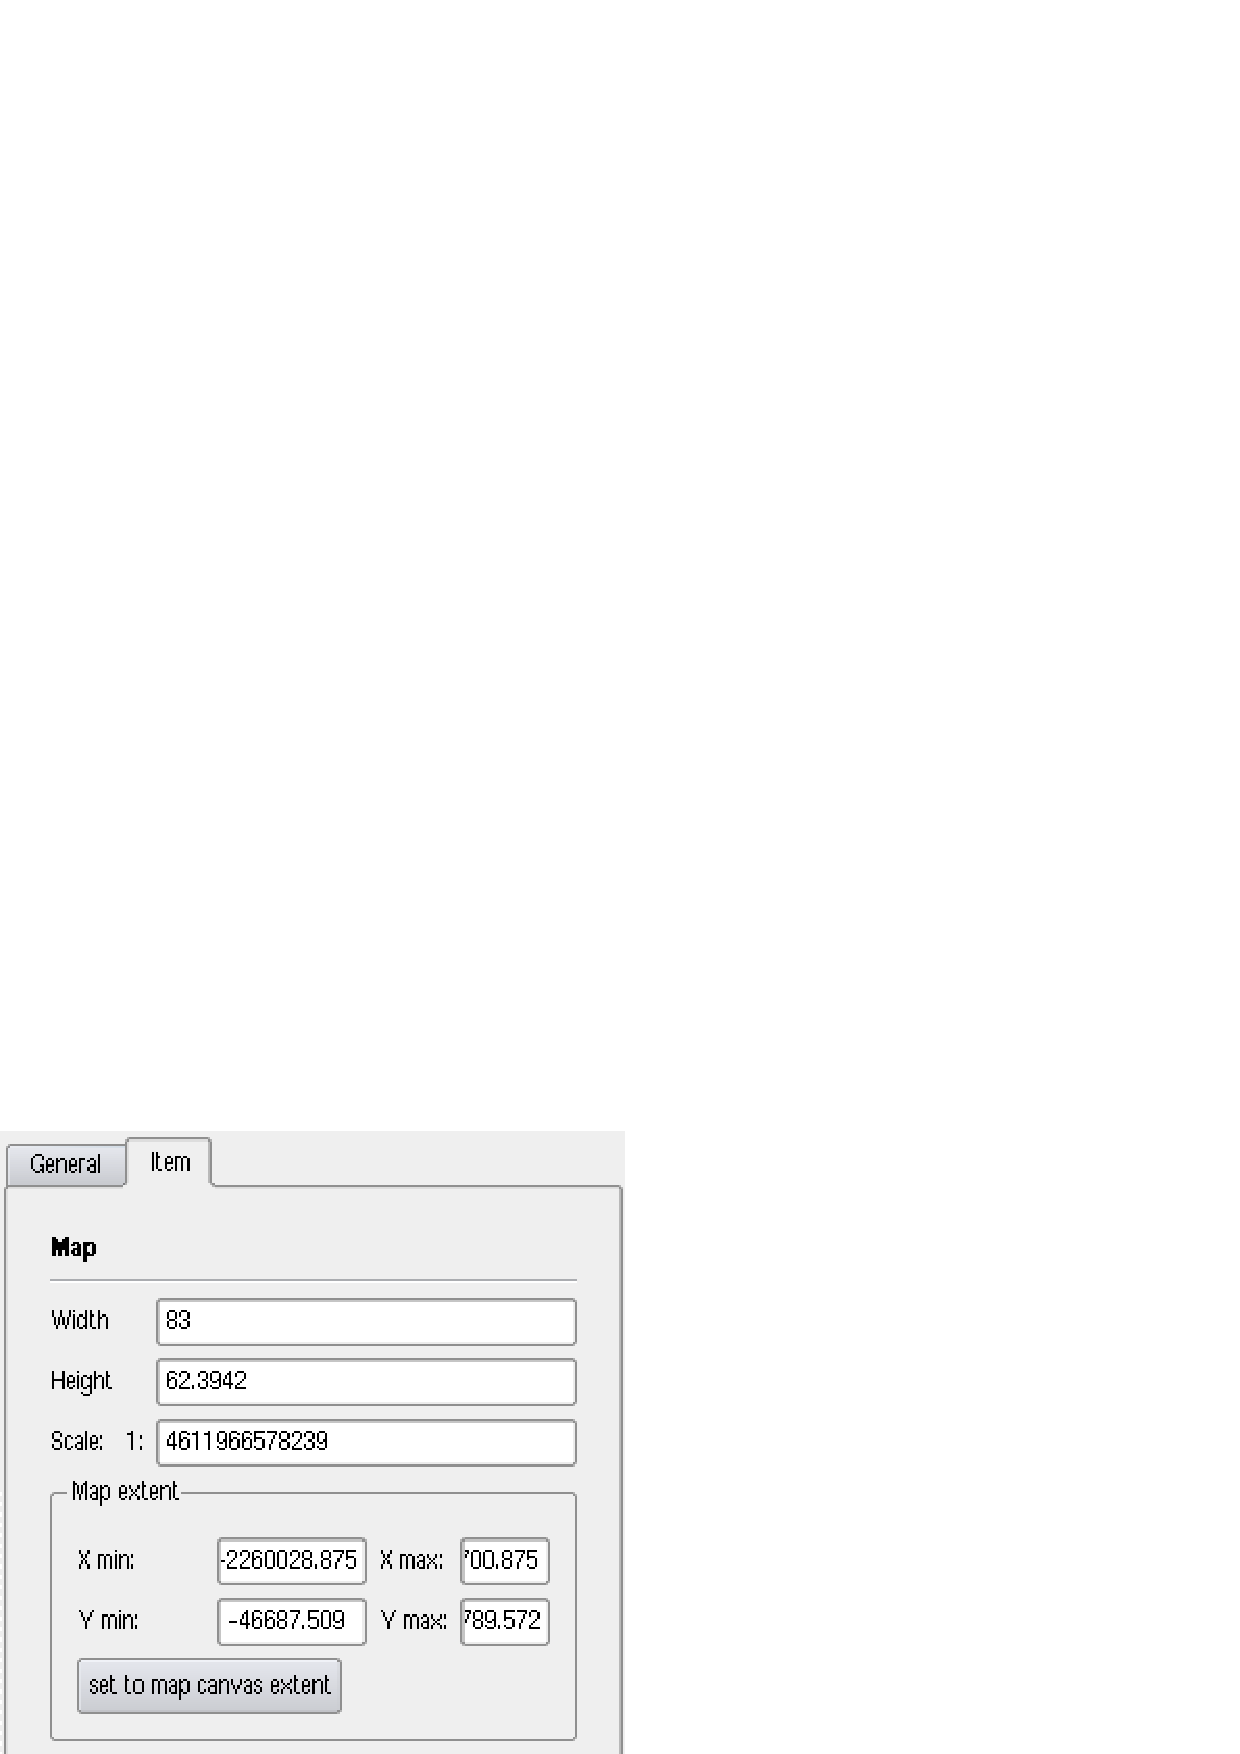
\includegraphics[clip=true,
width=0.4\textwidth]{print_composer_map_item1}}\goodgap
%    \subfigure[Properties dialog]
   \subfigure[Boîte de dialogue des
propriétés]{\label{subfig:print_composer_map_item2}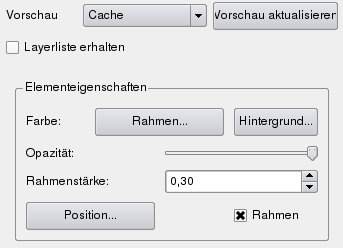
\includegraphics[clip=true,
width=0.4\textwidth]{print_composer_map_item2}}
\end{figure}

% You can resize the map later by clicking on the
% \toolbtntwo{mActionSelectPan}{Select/Move item} button, selecting the element,
% and dragging one of the blue handles in the corner of the map. With the map
% selected, you can now adapt more properties in the map \tab{Item} tab. Resize
% the map item specifying the width and height or the scale. Define the map
% extend using Y and X min/max values or clicking the \button{set to map canvas
% extend} button. Update the map preview and select, whether to see a preview
% from cache or an empty rectangle with a \textit{"Map will be printed here"}
% message. Define colors and outline width for the element frame, set a
% background color and opacity for the map canvas. And you can also select or
% unselect to display an element frame with the \checkbox{frame} checkbox 
% (see Figure~\ref{fig:print_composer_map_item}). If you change the view on the
% QGIS map canvas by zooming or panning or changing vector or raster properties,
% you can update the print composer view selecting the map element in the print
% composer and clicking the \button{Update Preview} button in the map \tab{Item}
% tab (see Figure~\ref{fig:print_composer_map_item}).
Vous pouvez redimensionner la carte plus tard en cliquant sur le bouton
\toolbtntwo{mActionSelectPan}{Sélectioner/Déplacer l'objet}, en sélectionnant
l'élément, et en déplaçant un des curseurs bleus dans le coin de la carte. Avec
la carte sélectionnée, vous pouvez maintenant adapter plus de propriétés dans
l'onglet \tab{Item} de la carte.

% To move layers within the map element select the map element, click 
% the \toolbtntwo{mActionMoveItemContent}{Move item content} icon and move the
% layers within the map element frame with the left mouse button.
Pour déplacer une couche dans l'élément 'carte', sélectionnez l'élément 'carte',
cliquez sur l'icône \toolbtntwo{mActionMoveItemContent}{Déplacer le contenu
de l'objet} et déplacez les couches dans le cadre de l'élément 'carte' avec le
bouton gauche de la souris.

% \begin{Tip}\caption{\textsc{Saving a print composer layout}}
\begin{Tip}\caption{\textsc{Sauver une mise en page du composeur de carte}}
% \qgistip{If you want to save the current state of a print composer session,
% click on \mainmenuopt{File} > \dropmenuopttwo{mActionFileSaveAs}{Save Project
% As} to save the state of your workspace including the state of the current
% print composer session. It is planned but currently not possible to save print
% composer templates itself.
\qgistip{Si vous voulez sauver l'état actuel de la session du composeur de
carte, cliquez sur \mainmenuopt{Fichier} >
\dropmenuopttwo{mActionFileSaveAs}{Sauvez le projet comme} pour sauver l'état
de votre espace de travail incluant l'état de la session actuelle du composeur
de carte. Il est prévu, mais actuellement pas possible de sauver les templates
du composeur de carte eux-mêmes.
}
\end{Tip} 

% \subsubsection{Adding other elements to the Print Composer}
\subsubsection{Ajouter d'autres éléments au Composeur d'Impression}

% Besides adding a current QGIS map canvas to the Print Composer, it is also
% possible to add, move and customize legend, scalebar, images and label
% elements.
Au-delà de l'ajout d'un cadre de la carte actuelle de QGIS au composeur de
carte, il est également possible d'ajouter, déplacer et personnaliser les
éléments légendes, échelles graphiques, images et étiquettes.

% \minisec{Label and images}
\minisec{Étiquette et images}

% To add a label or an image, click the \toolbtntwo{mActionLabel}{Add label} or 
% \toolbtntwo{mActionSaveMapAsImage}{Add image} icon and place the element 
% with the left mouse button on the print composer canvas.
Pour ajouter une étiquette ou une image, cliquez sur l'icône
\toolbtntwo{mActionLabel}{Ajouter une étiquette} ou
\toolbtntwo{mActionSaveMapAsImage}{Ajouter une image} et placez l'élément avec
le bouton gauche de la souris sur le cadre du composeur de carte.

\begin{figure}[ht]
\centering
% \caption{Customize print composer label and images
\caption{Personnaliser les étiquettes et les images du composeur de carte
\nixcaption}\label{fig:print_composer_tab2}
%    \subfigure[label item tab]
   \subfigure[onglet item des étiquettes]
{\label{subfig:print_composer_label_item}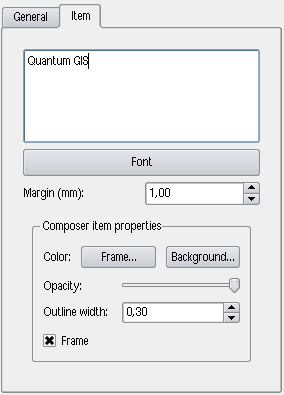
\includegraphics[clip=true,
width=0.4\textwidth]{print_composer_label_item}}\goodgap
%    \subfigure[image item tab]
   \subfigure[onglet item des images]
{\label{subfig:print_composer_image_item}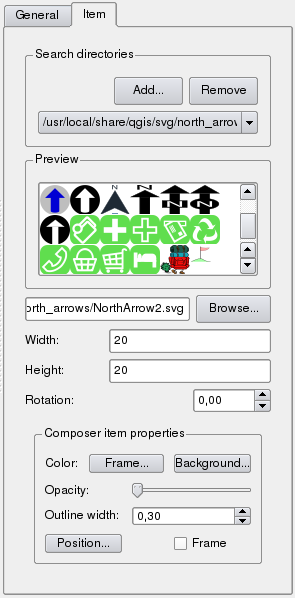
\includegraphics[clip=true,
width=0.4\textwidth]{print_composer_image_item}}
\end{figure}

% \minisec{Legend and scalebar}
\minisec{Légende  et barre d'échelle}

% To add a map legend or a scalebar, click the \toolbtntwo{mActionAddLegend}{Add
% new legend} or \toolbtntwo{mActionScaleBar}{Add new scalebar} icon and place
% the element with the left mouse button on the print composer canvas.
Pour ajouter une légende ou une échelle graphique, cliquez sur l'icône
\toolbtntwo{mActionAddLegend}{ajouter une nouvelle légende} ou
\toolbtntwo{mActionScaleBar}{Ajouter une nouvelle échelle graphique} et placez
l'élément avec le bouton gauche de la souris sur le cadre du composeur de carte.

\begin{figure}[ht]
\centering
% \caption{Customize print composer legend and scalebar
\caption{Personnaliser la légende et l'échelle graphique du composeur de carte
\nixcaption}\label{fig:print_composer_tab1}
%    \subfigure[legend item tab]
    \subfigure[onglet item de la légende]
{\label{subfig:print_composer_legend_item}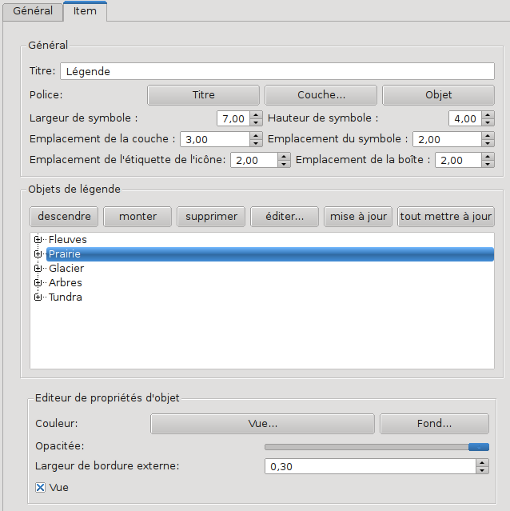
\includegraphics[clip=true,
width=0.4\textwidth]{print_composer_legend_item}}\goodgap
%    \subfigure[scalebar item tab]
   \subfigure[onglet item de l'échelle graphique]
{\label{subfig:print_composer_scalebar_item}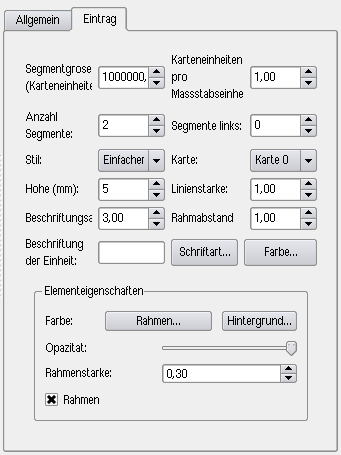
\includegraphics[clip=true,
width=0.4\textwidth]{print_composer_scalebar_item}}
\end{figure}

% \subsubsection{Navigation tools}
\subsubsection{Outils de navigation}

% For map navigation the print composer provides 4 general tools:
Pour la navigation de la carte le composeur de la carte fournie 4 outils
généraux :

\begin{itemize}
% \item \toolbtntwo{mActionZoomOut}{Zoom in},
\item \toolbtntwo{mActionZoomOut}{Zoomer},
% \item \toolbtntwo{mActionZoomOut}{Zoom out},
\item \toolbtntwo{mActionZoomOut}{Dézoomer},
% \item \toolbtntwo{mActionZoomFullExtent}{Zoom to full extend} and
\item \toolbtntwo{mActionZoomFullExtent}{Zoom à l'étendue maximale} et
% \item \toolbtntwo{mActionDraw}{Refresh the view}, if you find the view in an
% inconsistent state.
\item \toolbtntwo{mActionDraw}{Rafraîchir la vue}, si vous trouvez la vue dans
un état incomplet.
\end{itemize}

% \subsubsection{Creating Output}
\subsubsection{Création de carte}

% Figure \ref{fig:print_composer_complete} shows the print composer with an
% example print layout including each type of map element described in the
% sections above.
La figure \ref{fig:print_composer_complete} montre le composeur de carte avec
un exemple de mise en page incluant chaque type d'élément de la carte décrit
dans la section au-dessus.

\begin{figure}[h]
   \begin{center}
%    \caption{Print Composer with map view, legend, scalebar, and text added
\caption{Composeur de carte avec une vue de la carte, de la légende, de
l'échelle graphique et du texte ajouté
\nixcaption}
   \label{fig:print_composer_complete}\smallskip
   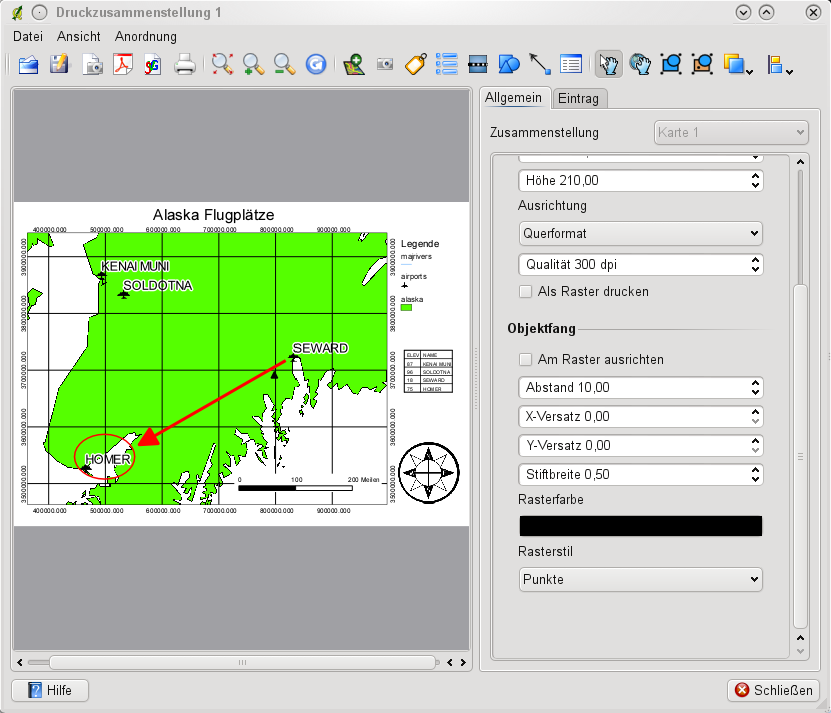
\includegraphics[clip=true, width=\textwidth]{print_composer_complete}
\end{center}
\end{figure}

% The print composer allows you to create several output formats and it is
% possible to define the resolution (print quality) and paper size:
Le composeur de carte vous permet de choisir plusieurs formats de sortie et il
est possible de définir la résolution (qualité d'impression) et la taille du
papier :

\begin{itemize}
% \item The \toolbtntwo{mActionFilePrint}{Print} icon allows to print the
% layout to a connected printer or as PDF or Postscript file depending on
% installed printer drivers.
\item L'icône \toolbtntwo{mActionFilePrint}{Imprimer}  permet d'imprimer la
mise en page à une imprimante ou dans un fichier PDF ou Postscript en fonction
des pilotes d'imprimante installée.
% \item The \toolbtntwo{mActionExportMapServer}{Export as image} icon exports
% the composer canvas in several image formats such as PNG, BPM, TIF, JPG, \dots
\item L'icône \toolbtntwo{mActionExportMapServer}{Exporter dans une image}
exporte le cadre du composeur dans plusieurs formats d'image tels que PNG, BPM,
TIF, JPG, \dots
% \item The \toolbtntwo{mActionSaveAsSVG}{Export as SVG} icon saves the print 
% composer canvas as a SVG (Scalable Vector Graphic). \textbf{Note:} Currently
% the SVG output is very basic. This is not a QGIS problem, but a problem of the
% underlaying Qt library. This will hopefully be sorted out in future versions.
\item L'icône \toolbtntwo{mActionSaveAsSVG}{Exporter au format SVG} sauve le
cadre du composeur de carte en SVG (Scalable Vector Graphic). \textbf{Note :}
Actuellement la sortie SVG est très basique. Ce n'est pas un problème de QGIS
mais un problème de la bibliothèque Qt sous-jacente. Cela sera
probablement corrigé dans une prochaine version.
\end{itemize}
